Partiendo de las bases descritas en la sección anterior la simulación consistirá, de forma general, en lanzar rayos y acumular los resultados de los receptores.

Aprovechando las ventajas de la programación orientada a objetos, se considerarán los siguientes clases:
\begin{itemize}
    \item \textbf{Rayo} Esta clase contendrá el punto de partida y el vector de dirección del rayo, así como la potencia en el origen.
    \item \textbf{Pared} En esta clase se incluirán los cuatro puntos de los extremos de la pared, a partir de los que se calculará su normal, también almacenada. Además, contendrá el valor de permeabilidad dieléctrica de su material.
    \item \textbf{Receptor} Esta clase incluye el origen de la esfera y su radio.
\end{itemize}

Las clases de las paredes y los receptores implementarán métodos que tengan de entrada un cierto rayo y que determinarán si habrá algún impacto entre ellos.

A la hora de almacenar los datos de los receptores no es posible acumular los valores de todos los rayos impactados ya que daría valores muy altos totalmente irreales.
El hecho de que muchos de los rayos impacten contra los receptores es fruto de la modelización como esfera, dando más volumen del que realmente tiene la esfera.

Por ello, se dividirá el reconocimiento de impactos dependiendo de los rebotes que haya recibido.
De esta forma se podrán separar los rayos que se reciben de forma directa de los rebotados.

A la hora de registrar la potencia recibida, para cada uno de los rebotes que ha sufrido el rayo, se elegirá aquel con una potencia mayor, al ser el que impacta de forma más directa con la esfera receptora, comportamiento buscado.

Estos valores se registrarán en una matriz en la que se considera a cada fila como cada receptor, y cada columna como estos valores de rebotes.
Así, tras finalizar la evaluación de rayos se acumularán todos los valores en cada fila, siendo el resultado final para cada receptor.

\begin{algorithm}
    \caption{Bucle Principal}
    \label{euclid}
    \begin{algorithmic}[1]
        \State Leer parámetros.
        \State Cargar mapa.
        \State Colocar receptores.
        \For{azimut $\in [0, 360)$}\Comment{Se evaluan los ángulos sumando un cierto paso fijado en los parámetros.}
            \For{elev $\in [90, -90]$}
                \State eval\_ray(azimut, elev, pot, data)
            \EndFor
        \EndFor

        \For{$i\gets 0, rows(data)$}
            \ForAll{$j\gets 1, cols(data)$}
                \State data[i][0] $\gets$ data[i][0] + data[i][j]
            \EndFor
        \EndFor

        \State write\_results(file, data)
    \end{algorithmic}
\end{algorithm}

\subsubsection*{Evolución de cada rayo}

El lanzamiento y evolución de cada rayo tiene varias fases a discutir.

En primer lugar, una vez se ha determinado la dirección de lanzamiento se debe calcular la potencia a emitir.
Habiendo importado la direccionalidad de la antena de emisión, se realiza una interpolación bidimiensional\footnote{En este caso esta interpolación ha sido bilineal. Aunque es posible obtener unos valores más precisos con métodos de mayor orden, partiendo de puntos separados solo un grado en ambos ángulos esta elección proporciona valores aceptables sin tener que abordar las condiciones de contorno en los extremos.} para determinar el valor exacto.

Como se comentaba en la sección del fundamento teórico, en cada impacto se generarán dos rayos.
Así, si este impacto llega a producirse, será necesario almacenar uno de los rayos producidos para ser evaluado más tarde.

Este almacenamiento se hará en forma de pila, de tal forma que los rayos añadidos más recientemente serán los primeros en ser evaluados.
Esta elección es totalmente arbitraria: todos los rayos son independientes entre sí.

Para optimizar el uso de memoria de la pila se reservará toda la memoria que se podría usar antes de iniciar el bucle y así no necesitar movimientos posteriores.
El tamaño necesario vendrá determinado por el número de rebotes que se quieran registrar.

% \begin{figure}[H]
%     \centering
%     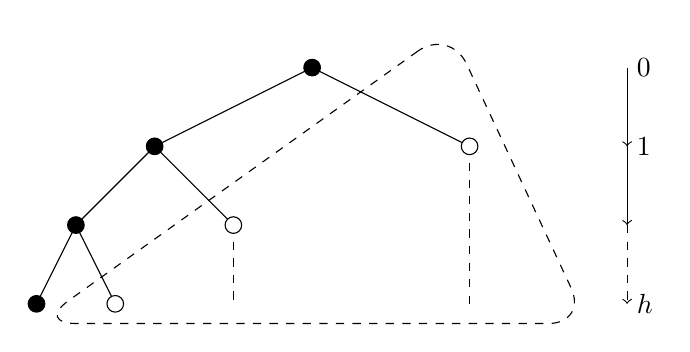
\begin{tikzpicture}

    % Conexiones
    \draw (0,0) -- (-2,-1);
    \draw (0,0) -- (2,-1);

    \draw (-2,-1) -- (-3,-2);
    \draw (-2,-1) -- (-1,-2);

    \draw (-3,-2) -- (-3.5,-3);
    \draw (-3,-2) -- (-2.5,-3);

    \draw[dashed] (2,-1) -- (2,-3);
    \draw[dashed] (-1,-2) -- (-1,-3);


    % Puntos
    \filldraw (0,0) circle [radius=3pt, fill=black];

    \filldraw (-2,-1) circle [radius=3pt, fill=black];
    \filldraw[draw=black, fill=white] (2,-1) circle [radius=3pt];

    \filldraw (-3,-2) circle [radius=3pt, fill=black];
    \filldraw[draw=black, fill=white] (-1,-2) circle [radius=3pt];

    \filldraw (-3.5,-3) circle [radius=3pt, fill=black];
    \filldraw[draw=black, fill=white] (-2.5,-3) circle [radius=3pt];

    % Niveles
    \draw[->] (4,0) -- (4,-1);
    \node[anchor=west] at (4,0) {0};

    \draw[->] (4,-1) -- (4,-2);
    \node[anchor=west] at (4,-1) {1};


    \draw[dashed, ->] (4,-2) -- (4,-3);
    \node[anchor=west] at (4,-3) {$h$};

    % Envoltorio

    \draw[dashed] [rounded corners=0.5cm] (1.75,0.5) -- (-3.5,-3.25)[rounded corners=0.5cm] -- (3.5,-3.25) -- cycle;


\end{tikzpicture}
% \end{figure}

En la Figura~\ref{fig:memoria_pila} se indica el árbol generado por un rayo, donde en cada impacto nacen dos rayos.
Considerando que siempre se evalúa el rayo reflejado --en esta representación, el camino de la izquierda-- podría parecer que se deberá reservar memoria para todos los rayos restantes, pero es posible un uso menor.

Los rayos guardados en la pila no son evaluados de forma inmediata, así que los rayos que se generan no se conocerán hasta que se llegue a su nodo.
Es decir, el número de rayos en la pila no llegará nunca a ser tan alto.


\begin{algorithm}
    \caption{Bucle que evalúa cada rayo}
    \label{euclid}
    \begin{algorithmic}[1]
        % \State Añadir pareja \{rayo inicial, 0\} a la pila.
        
        \While{Tamaño pila > 0}
            \State reb $\gets$ segundo valor de la pareja \{rayo, rebote\}.

            \ForAll{Paredes}
                \State hit\_dist $\gets$ INFINITY
                \State wall\_hit $\gets$ -1
                \If{Pared golpeada}
                    \If{dist < hit\_dist}
                        \State hit\_dist $\gets$ dist
                        \State wall\_hit $\gets$ pared
                    \EndIf
                \EndIf
            \EndFor

            \ForAll{Receptores}
                \State hit\_dist $\gets$ INFINITY
                \State power $\gets$ 0
                \If{Receptor golpeado}
                    \If{hit\_power > power and dist < hit\_dist}
                        \State hit\_power $\gets$ power
                    \EndIf
                \EndIf
            \EndFor

            \If{power > CUTOFF\_POWER AND reb < MAX\_REBOUND}
                \State \{rayo, rebote\} $\gets$ \{ rayo\_reflejado, reb+1\}
                \State Añadir \{ rayo\_transmitido, reb+1\} a la pila.
            \Else
                \State \{rayo, rebote\} $\gets$ último valor de la pila.
            \EndIf
        \EndWhile
    \end{algorithmic}
\end{algorithm}

\subsection{Implementación en paralelo}

El hecho de que los rayos lanzados sean independientes entre sí convierte en el bucle principal en el escenario perfecto para ser ejecutado de forma paralela, ya que cada iteración del bucle no se verá interrumpida por las demás.

Para esta paralelización se ha hecho uso de tarjetas gráficas, que cuentan con un gran número de núcleos de cómputo pero para las que hay que tener en cuenta su estructura de memoria.

En general, a la hora de paralelizar un algoritmo es necesario hacer duplicaciones de datos para evitar condiciones de carrera que proporcionen resultados erróneos.
En los casos de muy alta paralelización como este es posible encontrarse con ciertas limitaciones.

La tarjeta gráfica usada en este caso ha sido una Nvidia GTX1070, sobre la que es posible el uso de la librería de Nvidia CUDA.
Esta tarjeta cuenta con 1920 núcleos agrupados en ??? multiprocesadores.

La estrategia de paralelización consistirá en asignar un rayo a cada hilo, que contará con su matriz de datos correspondiente donde registrará los impactos para luego ser acumulada en los datos finales.

Las tarjetas gráficas agrupan sus hilos en bloques.
Los hilos que se encuentren en un mismo bloque pueden acceder a una cierta cantidad de memoria compartida de un acceso más rápido que la memoria global común.

Para reducir la necesidad de memoria y aprovechar esta característica la acumulación de los datos se producirá en dos fases: el cálculo de cada rayo --asignado a cada hilo-- volcará sus datos en la memoria compartida del bloque.
Una vez acaban todo los hilos del bloque, se acumulan los datos en la memoria global, donde se ha reservado espacio para cada bloque.

Debido a la herencia del uso de este tipo de dispositivos para trabajos de vídeo, es posible acceder a los hilos y bloques con dos índices, de forma similar a una matriz.
Esta característica será útil en este caso, en el que los rayos se lanzarán en torno a los dos ángulos de las coordenadas esféricas.

Así, se asociará la dirección $x$ al ángulo azimutal y la dirección $y$ a la elevación.

Queda determinar el número de hilos en cada bloque.
En general, la memoria disponible para su uso compartido es una cantidad baja.
En el caso de la tarjeta gráfica usada, es de 48 KB\cite{Nvidia}.

\begin{figure}[H]
    \centering
    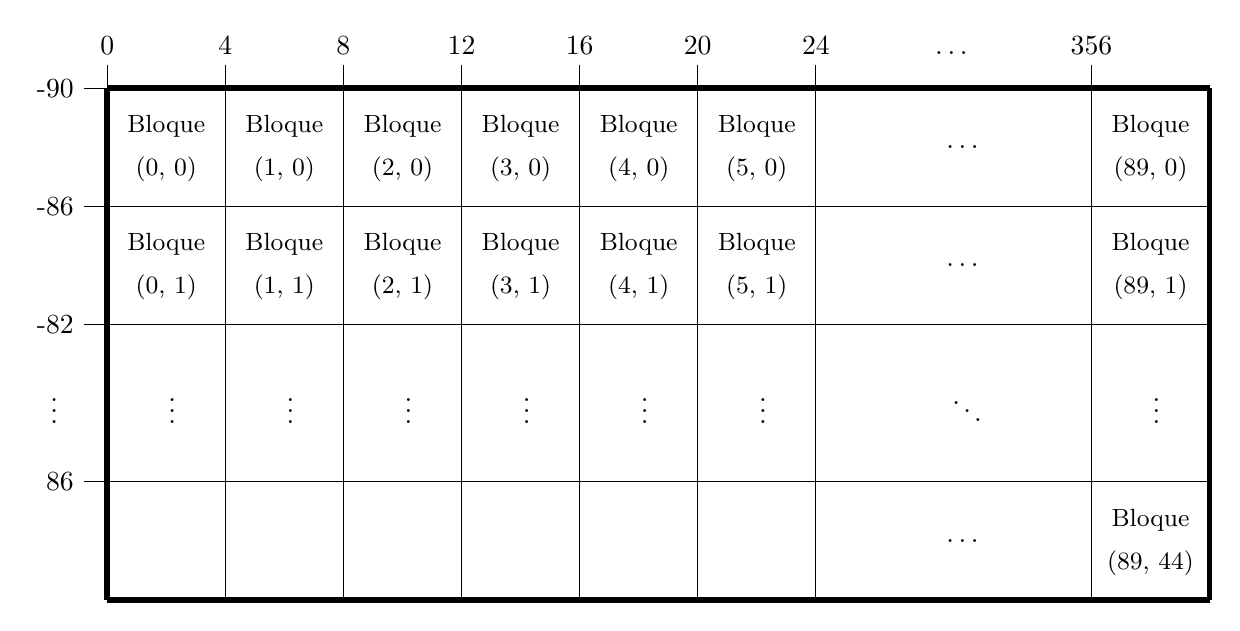
\begin{tikzpicture}
    \draw[line width=2pt] (0,0) -- (14,0);
    \draw[line width=2pt] (0,-6.5) -- (14,-6.5);
    \draw[line width=2pt] (0,0) -- (0,-6.5);
    \draw[line width=2pt] (14,0) -- (14,-6.5);

    % Labels
    \foreach \i in {0, 1.5, 3,...,10}
    {
        \draw (\i,0.3) -- (\i,-6.5);
        \pgfmathtruncatemacro{\label}{4*\i/1.5};
        \node[anchor=south] at (\i, 0.3) {\label \si{\degree}};
    }
    \draw (12.5,0.3) -- (12.5,-6.5);
    \node[anchor=south] at (12.5, 0.3) {356\si{\degree}};
    \node[anchor=south] at (10.75, 0.3) {\ldots};

    \foreach \i in {0, -1.5, -3}
    {
        \draw (-0.3, \i) -- (14, \i);
        \pgfmathtruncatemacro{\label}{90+4*\i/1.5};
        \node[anchor=east] at (-0.3, \i) {-\label \si{\degree}};
    }

    \draw (-0.3, -5) -- (14, -5);
    \node[anchor=east] at (-0.5, -4) {\vdots};
    \node[anchor=east] at (-0.3, -5) {86\si{\degree}};

    %Blocks
    \foreach \i in {1.5, 3, ...,10}
    {
        \pgfmathtruncatemacro{\bloquei}{\i/1.5 - 1};
        \foreach \j in {-1.5, -3}{
            \pgfmathtruncatemacro{\bloquej}{-\j/1.5-1};
            \node[anchor=south] at (\i-0.75, \j+0.75) {\small{Bloque}};
            \node[anchor=north] at (\i-0.75, \j+0.75) {\small{(\bloquei, \bloquej)}};

        }
        % \draw (\i,0.3) -- (\i,-6.5);
        % \pgfmathtruncatemacro{\label}{4*\i/1.5};
        
    }

    % Bloques extremo izquerda
    \node[anchor=south] at (13.25, -0.75) {\small{Bloque}};
    \node[anchor=north] at (13.25, -0.75) {\small{(89, 0)}};

    \node[anchor=south] at (13.25, -2.25) {\small{Bloque}};
    \node[anchor=north] at (13.25, -2.25) {\small{(89, 1)}};

    \node[anchor=south] at (13.25, -5.75) {\small{Bloque}};
    \node[anchor=north] at (13.25, -5.75) {\small{(89, 44)}};


    %Puntitos
    \foreach \i in {1.5, 3, ..., 10, 14}
    {
        \node[anchor=east] at (\i-0.5, -4) {\vdots};
    }

    \foreach \j in {0, -1.5, -5}
    {
        \node[anchor=east] at (11.25, \j-0.75) {\ldots};
    }

    \node[anchor=east] at (11.25, -4) {$\ddots$};


\end{tikzpicture}
    \caption{aa}
    \label{fig:CUDA_angulos}
\end{figure}

Esta cantidad no permite lanzar bloques con un número grande de hilos, aunque dependerá del número de receptores y los rebotes que se quieran registrar.
A modo de ejemplo, al colocar unos 40 receptores y registrar los rayos hasta 5 rebotes, con valores de precisión simple --es decir, 4 bytes--, podremos lanzar bloques con 60 hilos como máximo.

Para evitar futuras incompatibilidades en caso de elegir valores mayores en alguno de estos dos parámetros, se han elegido el mínimo valor de hilos posible.
La elección es la siguiente: solo se lanzarán 16 hilos por bloque, 4 en cada dirección.

Además de ser un valor bajo compatible con los límites establecidos, el número de ángulos a evaluar en ambas direcciones es divisible por 4, hecho aprovechable para la implementación.

La elección de asignación de valores angulares a los bloques será de forma fija: cada bloque solo evaluará 4 grados en cada dirección, independientemente del número de rayos que tenga asignado ejecutar.

Está claro que si la distancia entre los ángulos de un grado, cada hilo ejecutará el rayo con los ángulos que le corresponde sin más.
En el caso --habitual-- que la distancia sea menor, cada hilo deberá evaluar más de un rayo.

Para facilitar el recorrido y garantizar una ejecución lo más homogénea posible\footnote{Hay que tener en cuenta que la ejecución de los programas en tarjetas gráficas se realizan ejecutando una misma instrucción en varios hilos a la vez. Evitar expresiones condicionales que creen distintas ramas en el desarrollo del programa maximizará el rendimiento del dispositivo.}, solo se considerarán saltos en los valores angulares como potencias negativas de dos --es decir, solo se usarán saltos de valor $0.5$, $0.25$, $0.125$,...-- a fin de poder utilizar la siguiente estrategia.

Se considerará una matriz de «minibloques» dentro del bloque, todas ellas con los 16 hilos del bloque.
La cantidad de estos minibloques dependerá del valor del salto entre ángulos: si es $0.5 \equiv \sfrac{1}{2}$ habrá 4 minibloques, dos en cada dirección; si es $0.25 \equiv \sfrac{1}{4}$ habrá 16 minibloques, etc.

Dentro de cada uno de los minibloques solo habrá 16 pares de direcciones a evaluar, uno para cada hilo.
Una vez todos estos hilos finalicen su bucle, se avanzará al siguiente minibloque en dirección vertical --es decir, avanzando en el eje $y$-- hasta acabar con todos los ángulos que se deben evaluar.